\documentclass[12pt,a4paper]{article}
\usepackage[utf8]{inputenc}
\usepackage{amsmath}
\usepackage{amsfonts}
\usepackage{amssymb}
\usepackage{lmodern}
\usepackage[toc]{appendix}

\usepackage{graphicx}

\author{Noah Bergman}
\title{Heads-Up Display for a Manufacturing Microscope}
\begin{document}
\maketitle

\pagebreak



\tableofcontents

\listoffigures

\listoftables

\pagebreak
%%%%%%%%%%%%%%%%%%%%%%%%%%%%%%%%%%%%%%%%%%%%%%%%%%%%%%%%%%%%%%%%%%%%%%%%%%%%%%%%%
\section{Introduction}
Honeywell technicians assemble miniature mechanisms under a microscope. They face repetitive movements and eye strain while checking work instructions which are displayed on a nearby computer. A Kansas State design team outlined several solutions to this problem; a small tablet mounted next to the microscope, a virtual environment using technology similar to the Oculus Rift, and a heads up display inside the microscope’s field of view. We are exploring the last of these options. 





%%%%%%%%%%%%%%%%%%%%%%%%%%%%%%%%%%%%%%%%%%%%%%%%%%%%%%%%%%%%%%%%%%%%%%%%%%%%%%
\section{Project Statement}
Optically inserting a virtual screen inside the microscope’s field of view allows the operator to seamlessly refer to work instructions during assembly. This setup could potentially improve workplace ergonomics and reduce manufacturing time while ensuring all components meet Honeywell’s high quality expectations. 

\section{Design Requirements}

\begin{itemize}
	\item Allows users to interact with PDFs that contain embedded pictures, videos, and links to other work instructions.
	\item Does not obstruct the 15” vertical workspace below the objective lens.
	\item Does not restrict airflow in the workspace to maintain ISO Class 7 clean room standards.
	\item Remains in focus during normal microscope operation.
\end{itemize}

\section{Deliverables}
\begin{itemize}
	\item Design working prototype of heads-up display system.
	\item Provide all design documents, schematics, and code.
	\item Operations Manual to demonstrate how to setup and use the system.
	\item Future design manual that outlines improvements and ideas for development down the line.
\end{itemize}


%%%%%%%%%%%%%%%%%%%%%%%%%%%%%%%%%%%%%%%%%%%%%%%%%%%%%%%%%
\section{Functional Overview}
To meet all the requirements, our group designed a DLP projector with custom optics, hardware, and firmware. Our design is centered around the Texas Instruments’ DLP3010 chipset and uses the DLP3010 EVM optical engine and DLP controller board.  The entire system can be broken down into three main parts: main control board, DLP control board, and the optical system. These subsystems work together to display the final image inside the microscope. 



\subsection{Main Control Board}
The main control board was designed to take an HDMI input and convert the data to 24 bit RGB format which is fed directly to the DLP3438 display controller. The on-board microcontroller, MSP430F2274, serves as both a user interface hub and system coordinator. The power-on switch and navigation buttons are connected GPIOs. These inputs are configured in software trigger certain events in the projector. For example, the left and right buttons can be used to change screen size, zoom, and cropping while the power switch simply triggers all the initialization code to run. The MCU communicates with both the ADV7611 and the DLPC3438 over I2C. All the power for the system is routed through the main board. The 5V input is stepped down to 3.3V and 1.8V using buck regulators. 

\subsection{DLP Controller}
The DLP controller board was part of an evaluation kit from Texas Instruments. The board consists of the DLPC3438 display controller and the DLPA2005 PMIC/ LED driver. These two integrated circuits work in tandem to control the DLP3010, digital micro-mirror device.

\subsection{Optical System}
This optical engine uses three LEDs, red, green, and blue, to project a full color image. The light is combined and reflected off the DMD and out through the custom optical system. The optics we designed take the projected light, magnify, correct for aberrations, and finally collimate the image before it is sent into the infinity space of the microscope. The EMZ-8TRU has a camera port attachment that was removed and modified to change the direction of the beam splitter. This allowed the image to be reflected up through the eyepiece where the user can view the virtual screen.

\begin{figure}
	\centering
	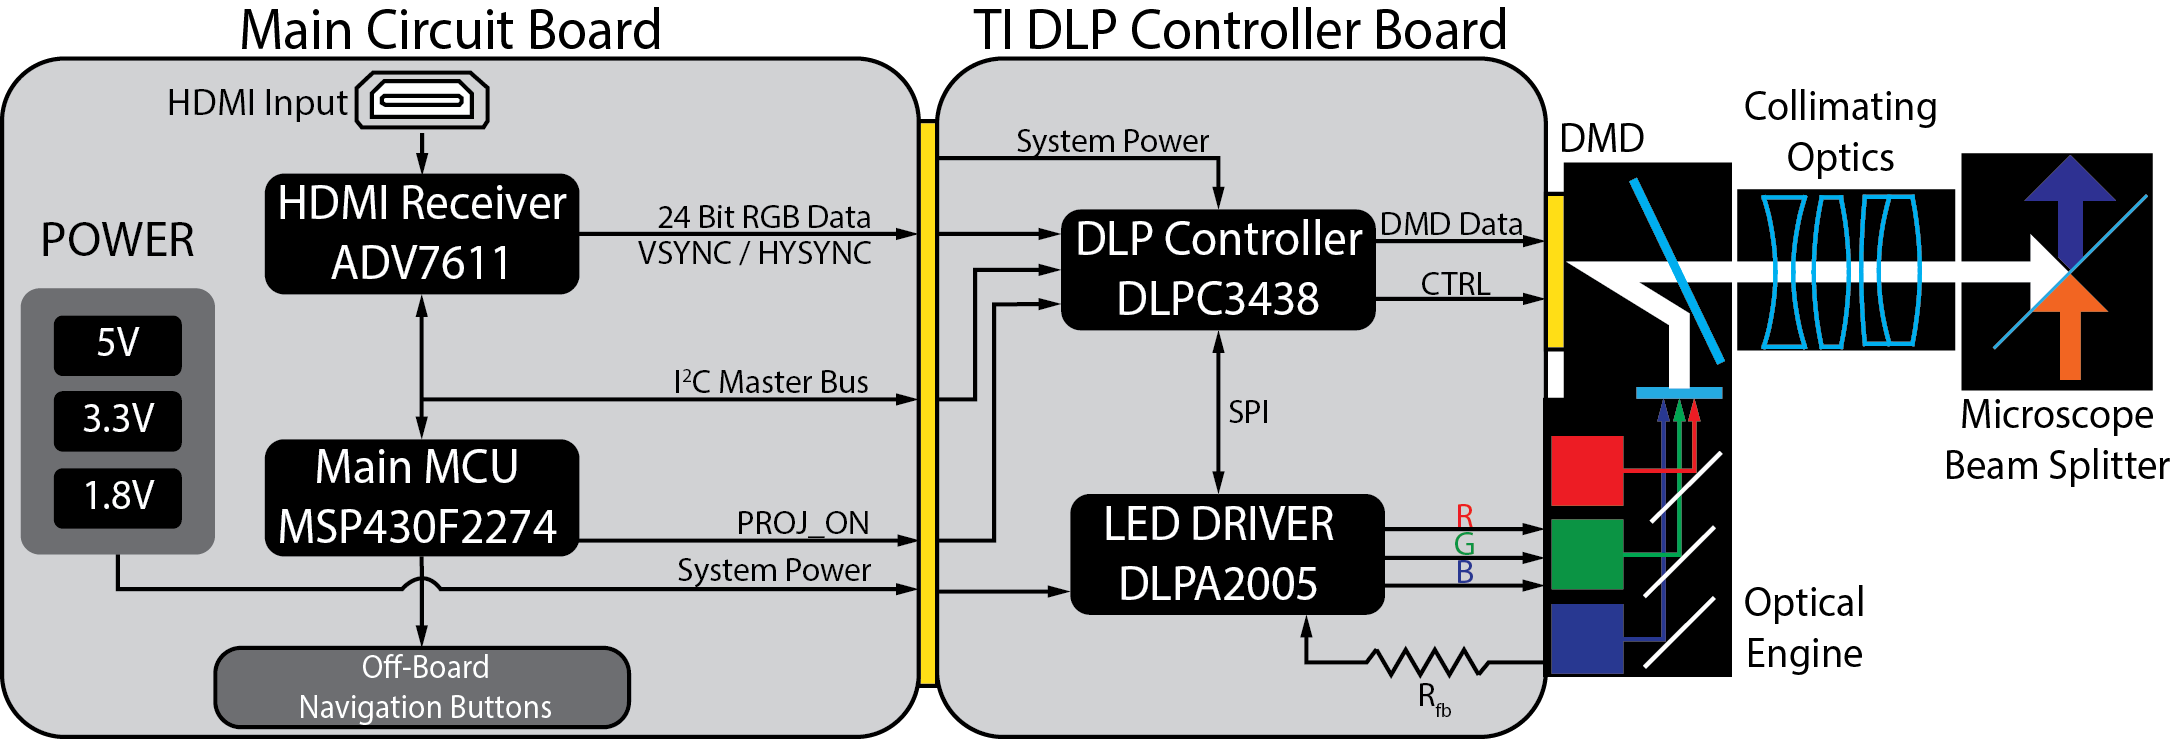
\includegraphics[width = \textwidth]{pics/seniorDesign_blockDiagram.png}
	\caption[Block Diagram]{Block diagram of the main board, DLP controller, and Optical system}
	\label{block_diagram}
\end{figure}




\section{Detailed Hardware Design}




%Double check on keeping here or in appendix -- The first design is
%not mentioned before this section -- necessarily
\section{Concept Comparison}



\section{Testing}




\section{Recommendations}





\section{Conclusion}






%Begin the appendix
\begin{appendices}

\section{Hello Appendix}

\end{appendices}
\end{document}